\subsection{\ref{str:sat} porovnání parametrů}\label{subsec:sat_porovnani_parametru}

U~\ref{str:sat} algoritmů jsem zkoušel stejné nastavení parametrů až na maximální počet prodlevu cesty (\ref{par:ars_mpc}),
jelikož musí být vždy nastaven na některou hodnotu.
Zjistil jsem, že složitost hledání roste velmi rychle se zvyšující \ref{par:ars_mpc},
proto jsem nastavil tento parametr maximálně na $24$.
I přes to měl algoritmus problémy.

S žádným nastavením mi algoritmy nedoběhly na velké křižovatce, pokud nepočítám neoptimalizovanou variantu.
Neoptimalizované běhy měli mnohem nižší čas plánování, avšak algoritmus mnoho agentů zamítal jen proto, že \ref{str:sat}
řešič vrátil model, který vjezd odmítl, i když by pro něj validní cesta existovala.
Proto jsem se rozhodl tento parametr nenastavovat, všechny zobrazené běhy jsou vyřešené \textrm{MAX-SAT}em.

\subsubsection{\nameref{subsec:sat_rsg} na \hyperref[par:data_mala]{malé} křižovatce}
\label{subsubsec:exp_satsg_mala_krizovatka}

\begin{table}[b!]
	\centering
%	\begin{adjustwidth}{-1.5cm}{}
	\begin{tabular}{c c c c | r r D{.}{,}{2.2} D{.}{,}{2.2} D{.}{,}{7.2}}
		\toprule \\
		\pulrad{\B{Typ}} & \pulrad{\B{Omez}} & \pulrad{\B{\ref{par:ars_mnv}}} &
		\pulrad{\B{\ref{par:ars_mpc}}} & \pulrad{\B{Krok}}  & \pulrad{\B{Zam}} &
		\mc{\pulrad{\B{pAg}}} & \mc{\pulrad{\B{pZp}}} & \mc{\pulrad{\B{Čas}}} \\
		\midrule
		S & - & 1 & 16 & 32782 & 1095     & \multicolumn{1}{B{.}{,}{2.2}}{14.29} & 5.99                                & \multicolumn{1}{B{.}{,}{7.2}}{4109.71}  \\
		S & s & 2 & 24 & 32778 & \B{255}  & 13.46                                & \multicolumn{1}{B{.}{,}{2.2}}{3.90} & 131515.34                               \\
		\hline
		O & - & 1 & 16 & 32784 & 4657     & 13.22                                & 8.65                                & \multicolumn{1}{B{.}{,}{7.2}}{15154.02} \\
		O & s & 2 & 24 & 32782 & \B{2868} & \multicolumn{1}{B{.}{,}{2.2}}{13.81} & \multicolumn{1}{B{.}{,}{2.2}}{7.77}  & 133605.81  \\
		\hline
		H & - & 1 & 16 & 32787 & \B{4403} & \multicolumn{1}{B{.}{,}{2.2}}{26.19} & 12.08                               & \multicolumn{1}{B{.}{,}{7.2}}{78214.86} \\
		H & s & 2 & 22 & 0     & 94573    & 1.02                                 & \multicolumn{1}{B{.}{,}{2.2}}{7.60} & 7200869.77                              \\
		\bottomrule
%		\multicolumn{6}{l}{\footnotesize \textit{Pozn:}
%		\textrm{Zam} - počet zamítnutí, \textrm{pAgen} - průměrný počet agentů v jeden krok na křižovatce, \\
%		\textrm{sAgen} - směrodatná odchylka počtu agentů na křižovatce, \\
%		\textrm{Zpož} - součet spoždění přes všechny agenty, \textrm{pZpož} - průměrné zpoždění agentů
%		}  TODO
	\end{tabular}
	\caption{Porovnání vlivu parametrů u \nameref{subsec:sat_rsg} na různých typech malé křižovatky.}\label{tab:sat_exp_mala}
%	\end{adjustwidth}
\end{table}


\ref{subsec:sat_rsg} se choval poměrně smysluplně, snižující omezení výpočtu vedlo k lepším výsledkům
za cenu vyšší doby plánování.
Tyto výsledky jsou v tabulce \ref{subsubsec:exp_satsg_mala_krizovatka}.

Jedinou výjimkou je hexagonální křižovatka, kde volnější varianta nespočítala skoro nic.

Je vidět vysoký nárůst složitosti při přechodu na graf s více vrcholy.
Opět si ale čtvercová křižovatka vedla mnohem lépe než hexagonální.

\subsubsection{\nameref{subsec:sat_ra} na \hyperref[par:data_mala]{malé} křižovatce}
\label{subsubsec:exp_sata_mala_krizovatka}

\ref{subsec:cbsoid} algoritmus ukazuje extrémní nárůst složitosti se zvyšujícím počtem plánovaných agentů.
Proto jsem značně snížil i \ref{par:ars_mpc}.

Výsledky jsou zapsané v tabulce \ref{tab:sata_exp_mala}.
Nejpřekvapivější jsou výsledky pro oktagonální křižovatku.
Nejprve mi přišlo zvláštní, že algoritmus, kterému vyšel nejnižší průměrný čas plánování nemá nejméně vypočtených kroků.
Podle mého je to způsobeno tím, že se \ref{str:sat} řešič na některém kroku zasekne a nepodaří se mu rozhodnout
určitý krok v čase, než uplynou dvě hodiny od počátku simulace.

\begin{table}[b!]
	\centering
%	\begin{adjustwidth}{-1cm}{}
	\begin{tabular}{c c c c c | r r D{.}{,}{2.2} D{.}{,}{1.2} D{.}{,}{8.2}}
		\toprule \\
		\pulrad{\B{Typ}} & \pulrad{\B{Omez}} & \pulrad{\B{\ref{par:ars_mnv}}} &
		\pulrad{\B{\ref{par:ars_mpc}}} & \pulrad{\B{\ref{par:aoid_mpa}}} & \pulrad{\B{Krok}} &
		\pulrad{\B{Zam}} & \mc{\pulrad{\B{pAg}}} & \mc{\pulrad{\B{pZp}}} & \mc{\pulrad{\B{Čas}}} \\
		\midrule
		S & - & 1 & 10 & 12 & 32776 & \B{363}   & \multicolumn{1}{B{.}{,}{2.2}}{15.07} & 5.44                                & \multicolumn{1}{B{.}{,}{8.2}}{9893.10}    \\
		S & - & 2 & 14 & 12 & 16634 & 32273     & 7.56                                 & \multicolumn{1}{B{.}{,}{1.2}}{4.58} & 432905.36                                 \\
		\hline
		O & - & 1 & 10 & 8  & 9289  & 47575     & \multicolumn{1}{B{.}{,}{2.2}}{15.16} & 8.74                                & 297656.39                                 \\
		O & s & 1 & 10 & 8  & 20821 & \B{25521} & \multicolumn{1}{B{.}{,}{2.2}}{15.16} & 8.57                                & 345728.00                                 \\
		O & s & 2 & 9  & 9  & 2740  & 59957     & 1.98                                 & 5.15                                & \multicolumn{1}{B{.}{,}{8.2}}{2632600.55} \\
		O & s & 2 & 9  & 10 & 99    & 65125     & 0.07                                 & \multicolumn{1}{B{.}{,}{1.2}}{3.07} & 30123061.30                               \\
		\hline
		H & - & 1 & 10 & 8  & 32788 & \B{1905}  & \multicolumn{1}{B{.}{,}{2.2}}{26.06} & 8.85                                & \multicolumn{1}{B{.}{,}{8.2}}{34920.59}   \\
		H & s & 2 & 12 & 8  & 11448 & 64109     & 9.30                                 & \multicolumn{1}{B{.}{,}{2.2}}{1.22} & 1240239.54                                \\
		\bottomrule
%		\multicolumn{6}{l}{\footnotesize \textit{Pozn:}
%		\textrm{Zam} - počet zamítnutí, \textrm{pAgen} - průměrný počet agentů v jeden krok na křižovatce, \\
%		\textrm{sAgen} - směrodatná odchylka počtu agentů na křižovatce, \\
%		\textrm{Zpož} - součet spoždění přes všechny agenty, \textrm{pZpož} - průměrné zpoždění agentů
%		}  TODO
	\end{tabular}
	\caption{Porovnání vlivu parametrů u \nameref{subsec:sat_ra} na různých typech malé křižovatky.}\label{tab:sata_exp_mala}
%	\end{adjustwidth}
\end{table}

\subsubsection{Závislost času plánování na zaplněnosti křižovatky}
\label{subsubsec:sat_zavislost_casu_a_agentu}

Všiml jsem si trochu zvláštního efektu při dělání experimentů se \ref{str:sat} algoritmy.
Čas plánování prvních pár kroků vždy trval příliš dlouho, ale s přibývajícími kroky se plánování zrychlovalo.
Potom jsem si uvědomil, že čím více je agentů na křižovatce, tím mají zbylí agenti méně možností, kde se nacházet.
To vede k vyššímu počtu výrokových proměnných, které musí být před startem řešiče \textrm{false}.
Tím pádem má řešič snadnější hledání nejlepších cest, jelikož má méně možných ohodnocení.

Abych tuto teorii více prozkoumal, vytvořil jsem dva grafy.
Oba grafy ukazují časy plánování a počet agentů na křižovatce pro jednotlivé kroky.
Data jsou zprůměrovaná přes určité sousední kroky, jelikož mají jednotlivé hodnoty,
obzvláště časy plánování, mají vysoký rozptyl.

První graf (Obrázek \ref{fig:cas_vs_agenti_satrsg}) ukazuje data pro oktagonální typ s použitím \nameref{subsec:sat_rsg}.

Tento běh měl povolené zastavování, \ref{par:ars_mnv} nastavený na $2$ a \ref{par:ars_mpc} na $24$.
Zvolil jsem tuto variantu, protože měla nejdelší průměrný plánovací čas.
Ale i přes to zde není výrazně vidět nepřímá úměra mezi časem a počtem agentů.

Nejspíše to je způsobeno tím, že pro více naplánovaných agentů se zároveň musí procházet více variant
při vytváření výrokových proměnných, čímž se zvyšuje čas přípravy před spuštěním řešiče.
Řešič poté najde ohodnocení relativně rychle, čímž příprava tvoří značnou část doby plánování.

\begin{figure}[h]
	\centering
	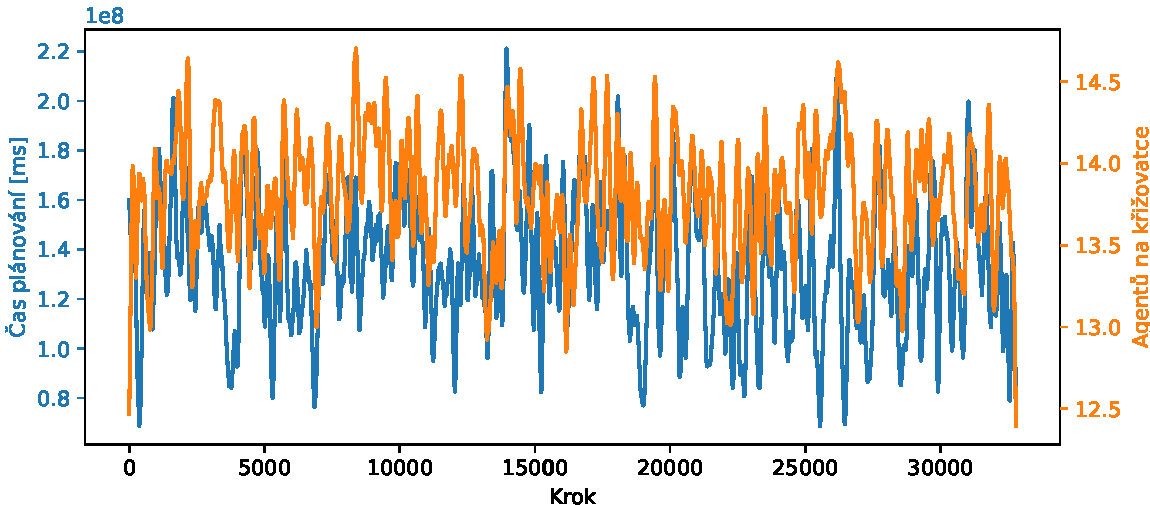
\includegraphics[width=140mm]{../img/CasVsAgentiSATRSG}
	\caption{Plánovací časy a počet naplánovaných agentů u \nameref{subsec:sat_rsg}}
	\label{fig:cas_vs_agenti_satrsg}
\end{figure}

Vytvořil jsem graf i pro \nameref{subsec:sat_ra} (Obrázek \ref{fig:cas_vs_agenti_satra}).
Tento běh byl taktéž z oktagonální křižovatky, kde algoritmus měl povolené zastavování,
\ref{par:ars_mnv} nastavené na $1$, \ref{par:ars_mpc} na $10$ a maximální počet plánovaných agentů byl $8$.

Dle mého názoru má zde mnohem větší vliv na plánování hledání modelu řešičem,
a proto je zde mnohem jasnější závislost mezi počtem agentů na křižovatce a časy plánování.
Obzvláště je zde vidět přibližně čtyřnásobná doba plánování v prvních krocích oproti průměrnému času.


\begin{figure}[h]
	\centering
	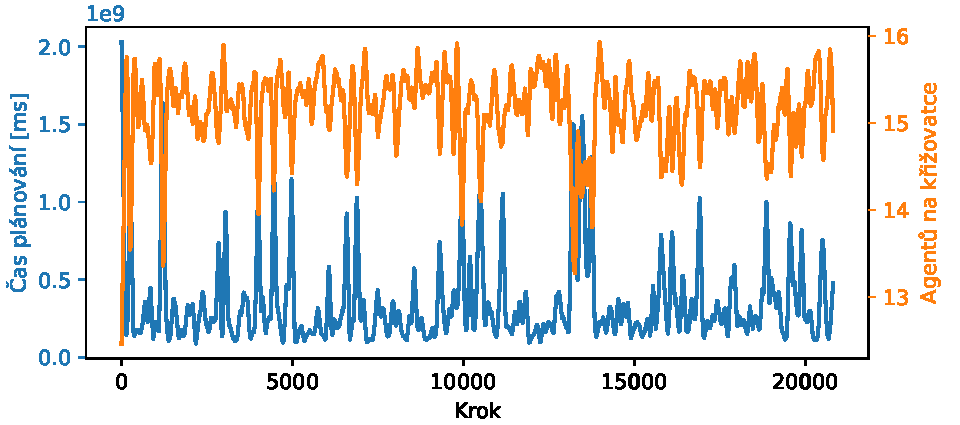
\includegraphics[width=140mm]{../img/CasVsAgentiSATRA}
	\caption{Plánovací časy a počet naplánovaných agentů u \nameref{subsec:sat_ra}}
	\label{fig:cas_vs_agenti_satra}
\end{figure}

